\documentclass[conference]{IEEEtran}
\IEEEoverridecommandlockouts
% The preceding line is only needed to identify funding in the first footnote. If that is unneeded, please comment it out.
\usepackage{cite}
\usepackage{amsmath,amssymb,amsfonts}
\usepackage[latin5]{inputenc}% For Turkish characters
\usepackage{algorithmic}
\usepackage{graphicx}
\usepackage{textcomp}
\usepackage{xcolor}
\usepackage{graphicx}% Include figure files
\usepackage{dcolumn}% Align table columns on decimal point
\usepackage{bm}% bold math
\usepackage[latin5]{inputenc}% For Turkish characters
\usepackage{amssymb}
\usepackage{amsmath}
\usepackage{amsthm}
\usepackage{amsbsy}
%\usepackage{mathptmx}
\usepackage{amsfonts}
\usepackage{mathtools}
\usepackage{physics}
\DeclareMathAlphabet{\mathcal}{OMS}{cmsy}{m}{n}
\usepackage{tabularx}
\usepackage{xcolor}
\usepackage{mathtools}
\usepackage{oubraces}
\usepackage{dsfont}
\usepackage{graphicx}
\usepackage{rotating}
\usepackage[most]{tcolorbox}
\usepackage{enumerate}
\usepackage{subfloat}
%\usepackage{hyperref}% add hypertext capabilities
\usepackage[colorlinks=true,linkcolor=blue,citecolor=blue,urlcolor=blue]{hyperref}%
\usepackage{cleveref}
\usepackage[normalem]{ulem}
\def\BibTeX{{\rm B\kern-.05em{\sc i\kern-.025em b}\kern-.08em
    T\kern-.1667em\lower.7ex\hbox{E}\kern-.125emX}}


\DeclarePairedDelimiter\ceil{\lceil}{\rceil}
\DeclarePairedDelimiter\floor{\lfloor}{\rfloor}

\begin{document}

\title{Deep Learning Project Progress Report}

\author{\IEEEauthorblockN{1\textsuperscript{st} H\"useyin Talha \c{S}enya\c{s}a}
\IEEEauthorblockA{\textit{Department of Physics, Faculty of Science and Letters,} \\
\textit{Istanbul Technical University,}\\
34469 Maslak, Istanbul, Turkey, \\
senyasa@itu.edu.tr}
}

\maketitle

\begin{abstract}

\end{abstract}

\begin{IEEEkeywords}
algorithmic trading, deep Learning, deep reinforcement learning.
\end{IEEEkeywords}

\section{Introduction}

\section{Implementation of the Framework}

In this section, we provide the details of the algorithmic trading framework. The framework consists of three main parts: Trading Environment, feed forward neural network and Double-Q mechanism. In this progress report, we provide the full detail of the trading environment which the RL agent interacts with, and then briefly report general structure of the remaining parts which are going to be implemented as a next step. 
 

\subsection{Trading Environment}

The nature of an environment in deep reinforcement learning applications is dictated by the problem in question. Although a trading action can be realized in a continuos medium i.e., a trading decision can be made at any time (e.g., based on a continuous function derived from a statistical model), algorithmic trading actions occurs in a discrete medium due to nature of the data to be processed.  In our case, the medium of the environment consists of discrete time series which is indexed by time step \(t\). The interval between sequential data points (corresponding to \(t-1\) and \(t\)) is determined by the trading frequency and it is denoted by \(\Delta t\). Since we only consider daily trading in this project, the interval \(\Delta t\) is equal to 1 day. 

\begin{figure}\label{fig:OHLCVfig}
    \centering
    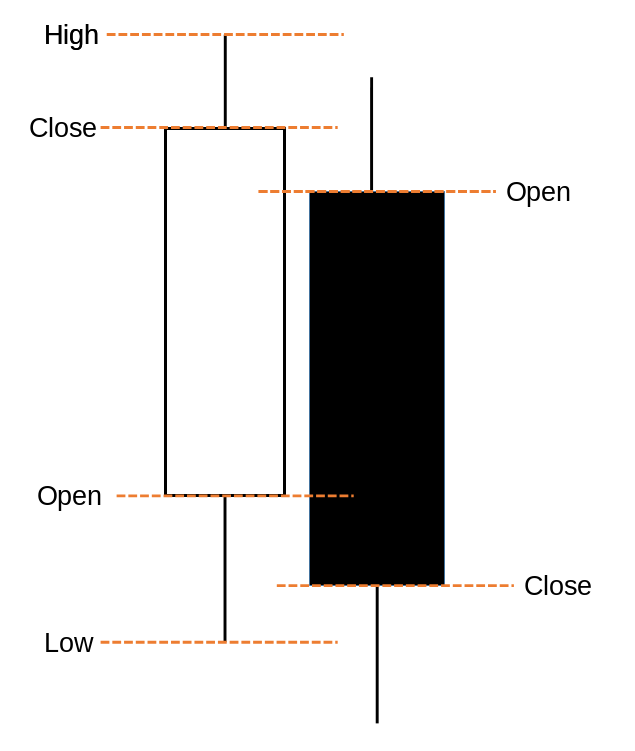
\includegraphics[scale=0.4]{Figs/Figures/OHLCV-Single.png}
    \caption{A diagram of candlestick chart of \textit{Open, High, Low, Close} for two sequential data points \(t\) (left white) and \(t+1\) (right black). Realize that the Open and Close labels are inverted in black candle. A white color candle represent an increase with respect to the opening price that is  \(\text{Close} > \text{Open} \), while a black candle represent a decrease with respect to the opening price that is \(\text{Close} < \text{Open} \). The \textit{wicks} (the above and below vertical lines) represent High and Low values of the stock over the period of \(\Delta t\) respectively for both candles.} 
\end{figure}

The trading environment consists of three parts: Data retrieval, trading operations and RL agent interface. To be able to built the trading environment, one must first obtain the required data regarding the stock in question. Here, we use an open source third party \textit{Yahoo Finance} python interface to retrieve the classical OHLCV (\textit{Open, High, Low, Close, Volume}) data of the stock. This set of information can be expressed as 
\begin{equation}\label{eq:OHLCVset}
    \mathcal{D}_t = \left\{p_{t}^O, p_{t}^H, p_{t}^L, p_{t}^C, V_{t} \,| \, t \in [t_i, t_f]\right\},
\end{equation}
where 
\begin{enumerate}[-]
    \item \(p_t^O\) is the opening price of over the period \([t - \Delta t, t]\),
    \item \(p_t^H\) is the highest price over the period \([t - \Delta t, t]\),
    \item \(p_t^H\) is the lowest price over the period \([t - \Delta t, t]\),
    \item \(p_t^C\) is the closing price over the period \([t - \Delta t, t]\),
    \item \(V_t\) is the total volume of shares exchange over the period \([t - \Delta t, t]\),
\end{enumerate}
where \(t_i\) and \(t_f\) are initial and final trading days respectively (see Fig.~\ref{fig:OHLCVfig}). After that, one needs to implement trading operations (whose details is given in the next section) to be able to execute trading decisions. Finally, one needs to implement RL agent interface to train the deep neural network. 

\begin{figure}
    \centering
    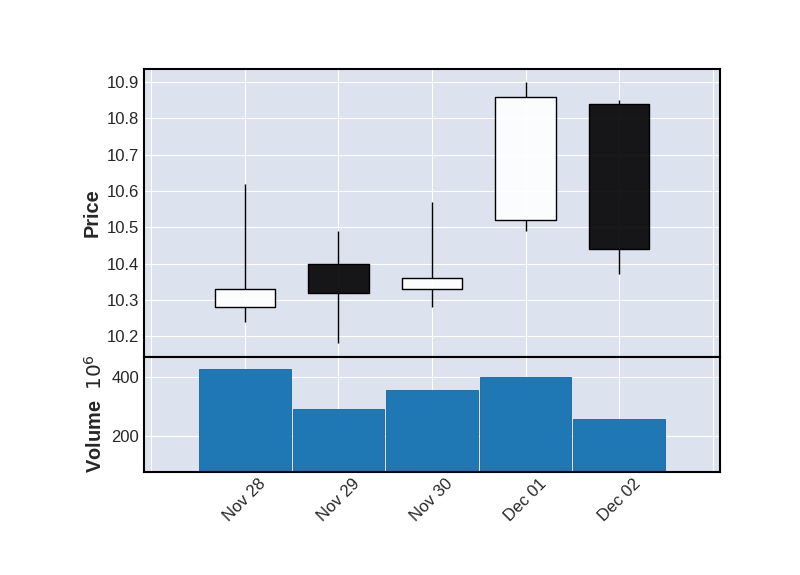
\includegraphics[scale=0.4]{Figs/Figures/OHLCV.png}
    \caption{A candlestick chart of \textit{Open, High, Low, Close}, for AAPL (Apple) stock with \textit{Volume} information for five days. Here, a volume bar represents the total number of shares exchange during the corresponding interval.}
\end{figure}


\subsubsection{Description of Trading Operations / Action Space}
Trading operations correspond to the actions that are available to the RL agent. The agent can buy or sell shares of the stock which translates into \textit{going long} and \textit{going short} respectively.  However, the RL agent must also decide the amount of shares it is going to buy or sell for a given time step \(t\) based on its portfolio e.g., \textit{cash} and \textit{number of shares}. To formally express the operations, we first define various quantities. Let \(C_{t} \in \mathds{R}^{\geq 0}\) be the available amount of \textit{cash} at time step \(t\) and then let \(Q_t \in \mathds{R}\) be the number of shares exchanged at time step \(t\). Positive values of \(Q_t\) means that the agent buys shares i.e., \textit{taking long action}, on the other hand, negative values of \(Q_t\) means selling shares i.e., \textit{taking short action} while \(Q_t = 0\) corresponds to holding position. However, during the implementation of the agent, we eliminate \(Q_t = 0\) case (that is, the agent only decides whether to buy or sell), by handling the position transition in a way that the same sequential action corresponds to \textit{hold} position. Therefore, the complete action space over all time steps \(t\) can be defined as
\begin{equation}
    \mathcal{A}_t = \{Q^{\text{Long}}_{t}, Q^{\text{Short}}_{t} \,| \, t \in [t_i, t_f]\}.
\end{equation}
where \(t_i\) and \(t_f\) are initial and final trading time steps respectively.


The agent starts its trading activity with an initial \(C_{t=t_i}\) amount of money and it is chosen in such a way that it is much lower than the average exchange volume of the stock in question. In this way, it becomes safe to assume that the trading actions carried out by the agent does not influence the stock movements. At a time step \(t\), the agent takes an action \(a_t \in \mathcal{A}_t\) which effects the portfolio, that is, it effects the available cash \(C_t\) and the number of shares \(n_t\) owned by the agent. Their update rules are defined as
\begin{equation}\label{eq:portfolio-update}
    C_{t+1} = C_t - Q_t p_{t}^{c} - F \abs{Q_t} p_{t}^{c}
\end{equation}
\begin{equation}
    n_{t+1} = n_t + Q_t
\end{equation}
where \(F\) denotes the trading cost. For a day trading, it is generally \(0.2\,\%\) of the exchange. We use this value as a trading cost. We would like to stress that the number of shares at a time step \(t\) (\(n_t\)) owned by the agent can have negative values. This negative quantity corresponds to the shares borrowed and sold. In fact, this operation is the actual meaning of the short position. However, the number of shares to be borrowed is calculated in a way that, the agent can repay the borrowed shares (i.e., \(C_{t} \gg Q_t^{\text{Short}} p_t^{C}\)).  

Having defined the update rules for cash and and the number of shares owned at a time step \(t\), we now can define the rule for the number of shares to be bought and sold at a time step \(t\). Although we may let the RL agent to decide this quantity, we supply a formula to the agent for simplicity.  Let \(C_t\) be the available cash at time step \(t\) and let \(Q_t\) be the number of shares the agent is going to buy or sell. If the agent takes the long position at time step \(t\), the agent will have 
\begin{equation}\label{eq:longaction}
    Q_t^{\text{Long}} =
    \begin{cases}
        \floor*{\dfrac{C_{t}}{p_t^C (1 + F)}} \, &\text{if} \,\, a_{t-1} \neq Q_{t-1}^{\text{Long}}, \\[15pt]
        0 \, &\text{otherwise}.
    \end{cases}
\end{equation} 
amount of shares. On the other hand, if the agent takes a short position at a time step \(t\)
\begin{equation}
    Q_t^{\text{Short}} =
    \begin{cases}
        -2 n_t - \floor*{\dfrac{C_{t}}{p_t^C (1 + F)}} \, &\text{if} \,\, a_{t-1} \neq Q_{t-1}^{\text{Short}}, \\[15pt]
        0 \, &\text{otherwise}.
    \end{cases}
\end{equation} 
amount of shares. 


\subsubsection{Implementation of Trading Operations}



One first needs to implement the trading operations to be able to implement the trading environment. The trading operations correspond to the actions that is taken by the agent. In normal circumstances, there must be a match between bid and ask orders to realize a trade operation. In order to detect these matches, one must be able access the order book of the stock in question. However, since assume that the total number of buy and sell orders are much smaller than the volume of the stock, we are going to implement only buy and sell operations. 

The trading operations are implemented in an object oriented manner. There are two main classes to control trading operations: \textit{StockHandler} and \textit{DummyPosition}. 

The StockHandler class obtains the stock data from \(\textit{Yahoo Finance}\) and applies minor transformations to eliminate possible missing data points. This class also responsible for the real-time tracking of the stock via \textit{Update} method. 


The DummyPosition class is implemented to carry out possible actions i.e., \textit{long} or \textit{short} operations. and to keep track of the position changes. While the information regarding the stock in question is handled by the StockHandler class, the DummyPosition class also stores the deep copy of the stock information to enable various data augmentation and manipulation. The two main methods of this class which correspond to the action of the RL agent are \textit{GoLong(.)} and \textit{GoShort(.)}. Both methods execute the given action then computes and updates the current value of the portfolio and the return with respect to the previous position which are used by the RL agent to take the next action.


\subsubsection{Implementation of Trading Environment via OpenAI Gym}

The environment which the deep learning agent interacts with is implemented by utilizing \textit{OpenAI Gym} framework. OpenAI Gym is an open source python library that provides standardized application programming interface (API) to establish interaction/communication between agents and environments for reinforcement learning problems. 

A third party application has to implement/override several functions/methods that are inherited from the \textit{gym} base class. These methods include initialization, iteration and reset of the environment in question. In the initialization part, one first builds the environment. In our case, it is the first \(\tau\) days starting from \(t_i\) due to the fact that the data we are processing have a sequential nature (Here \(\tau\) is a hyper-parameter of the framework, its details will be given in the reinforcement section). This initialized state which is denoted by \(S_{t=t_i}\) corresponds to current status of the environment. In the iteration part, first, the RL agent provides an \textit{action} to take, then, the environment state is transitioned to the next state according to the action provided by the RL agent. The iteration part can continue until a \textit{done} signal generated by the environment. In our case, the \textit{done} signal is generated when the iteration index becomes equal to \(t_f\). When a \textit{done} signal is produced one needs to \textit{reset} the environment. In the \textit{reset} part, one simply deletes all memory of the agent and supplies it with a new environment. (One may question that in such a case, after a reset the RL agent would execute the same action. However, a randomness is introduce to prevent this loop. Details will be given in the reinforcement section).

\begin{figure}
    \centering
    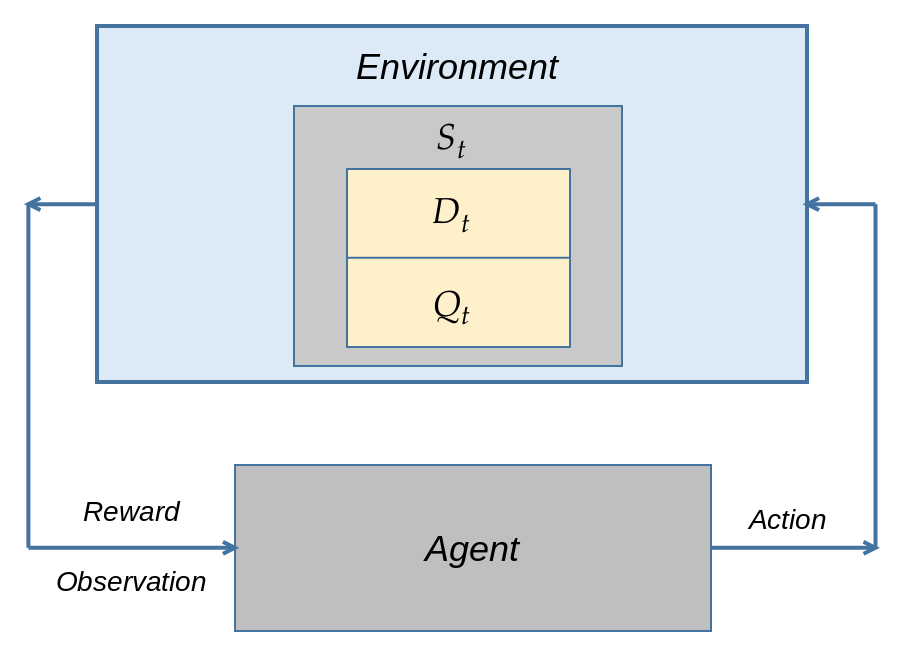
\includegraphics[scale=0.35]{Figs/Figures/TradeEnvironment.png}
    \caption{Diagram of the trading environment and agent relation. Here, \(S_t\) is the state of the environment at time step \(t\), \(D_t\) is given in Eq.~\eqref{eq:OHLCVset}, and \(Q_t\) is the position at time step \(t\). The trading environment framework first initializes the environment with \(D_{t=t_i}\) and then the agent observes the environment and provides an action \(a_{t_i} \in \mathcal{A}_t\). After that the environment transitions to \(S_{t} \rightarrow S_{t+1}\) accordingly. This process is repeated until a \textit{done} is generated by the environment.} 
\end{figure}


\end{document}
